\chapter{Chapter XIII}

\begin{verse}
``Heroes, approach!'' Atrides thus aloud,\\
``Stand forth distinguish'd from the circling crowd,\\
Ye who by skill or manly force may claim,\\
Your rivals to surpass and merit fame.\\
This cow, worth twenty oxen, is decreed,\\
For him who farthest sends the winged reed.''\\!
\attrib{--Iliad}
\end{verse}

\lettrine{T}{he} name of Ivanhoe was no sooner pronounced than it flew
from mouth to
mouth, with all the celerity with which eagerness could convey and
curiosity receive it. It was not long ere it reached the circle of the
Prince, whose brow darkened as he heard the news. Looking around him,
however, with an air of scorn, ``My Lords,'' said he, ``and especially
you, Sir Prior, what think ye of the doctrine the learned tell us,
concerning innate attractions and antipathies? Methinks that I felt the
presence of my brother's minion, even when I least guessed whom yonder
suit of armour enclosed.''

``Front-de-Boeuf must prepare to restore his fief of Ivanhoe,'' said De
Bracy, who, having discharged his part honourably in the tournament, had
laid his shield and helmet aside, and again mingled with the Prince's
retinue.

``Ay,'' answered Waldemar Fitzurse, ``this gallant is likely to reclaim
the castle and manor which Richard assigned to him, and which your
Highness's generosity has since given to Front-de-Boeuf.''

``Front-de-Boeuf,'' replied John, ``is a man more willing to swallow
three manors such as Ivanhoe, than to disgorge one of them. For the
rest, sirs, I hope none here will deny my right to confer the fiefs of
the crown upon the faithful followers who are around me, and ready to
perform the usual military service, in the room of those who have
wandered to foreign Countries, and can neither render homage nor service
when called upon.''

The audience were too much interested in the question not to pronounce
the Prince's assumed right altogether indubitable. ``A generous
Prince!--a most noble Lord, who thus takes upon himself the task of
rewarding his faithful followers!''

Such were the words which burst from the train, expectants all of them
of similar grants at the expense of King Richard's followers and
favourites, if indeed they had not as yet received such. Prior Aymer
also assented to the general proposition, observing, however, ``That the
blessed Jerusalem could not indeed be termed a foreign country. She was
`communis mater'--the mother of all Christians. But he saw not,'' he
declared, ``how the Knight of Ivanhoe could plead any advantage from
this, since he'' (the Prior) ``was assured that the crusaders, under
Richard, had never proceeded much farther than Askalon, which, as all
the world knew, was a town of the Philistines, and entitled to none of
the privileges of the Holy City.''

Waldemar, whose curiosity had led him towards the place where Ivanhoe
had fallen to the ground, now returned. ``The gallant,'' said he, ``is
likely to give your Highness little disturbance, and to leave
Front-de-Boeuf in the quiet possession of his gains--he is severely
wounded.''

``Whatever becomes of him,'' said Prince John, ``he is victor of the
day; and were he tenfold our enemy, or the devoted friend of our
brother, which is perhaps the same, his wounds must be looked to--our
own physician shall attend him.''

A stern smile curled the Prince's lip as he spoke. Waldemar Fitzurse
hastened to reply, that Ivanhoe was already removed from the lists, and
in the custody of his friends.

``I was somewhat afflicted,'' he said, ``to see the grief of the Queen
of Love and Beauty, whose sovereignty of a day this event has changed
into mourning. I am not a man to be moved by a woman's lament for her
lover, but this same Lady Rowena suppressed her sorrow with such dignity
of manner, that it could only be discovered by her folded hands, and her
tearless eye, which trembled as it remained fixed on the lifeless form
before her.''

``Who is this Lady Rowena,'' said Prince John, ``of whom we have heard
so much?''

``A Saxon heiress of large possessions,'' replied the Prior Aymer; ``a
rose of loveliness, and a jewel of wealth; the fairest among a thousand,
a bundle of myrrh, and a cluster of camphire.''

``We shall cheer her sorrows,'' said Prince John, ``and amend her blood,
by wedding her to a Norman. She seems a minor, and must therefore be at
our royal disposal in marriage.--How sayst thou, De Bracy? What thinkst
thou of gaining fair lands and livings, by wedding a Saxon, after the
fashion of the followers of the Conqueror?''

``If the lands are to my liking, my lord,'' answered De Bracy, ``it will
be hard to displease me with a bride; and deeply will I hold myself
bound to your highness for a good deed, which will fulfil all promises
made in favour of your servant and vassal.''

``We will not forget it,'' said Prince John; ``and that we may instantly
go to work, command our seneschal presently to order the attendance of
the Lady Rowena and her company--that is, the rude churl her guardian,
and the Saxon ox whom the Black Knight struck down in the tournament,
upon this evening's banquet.--De Bigot,'' he added to his seneschal,
``thou wilt word this our second summons so courteously, as to gratify
the pride of these Saxons, and make it impossible for them again to
refuse; although, by the bones of Becket, courtesy to them is casting
pearls before swine.''

Prince John had proceeded thus far, and was about to give the signal for
retiring from the lists, when a small billet was put into his hand.

``From whence?'' said Prince John, looking at the person by whom it was
delivered.

``From foreign parts, my lord, but from whence I know not'' replied his
attendant. ``A Frenchman brought it hither, who said, he had ridden
night and day to put it into the hands of your highness.''

The Prince looked narrowly at the superscription, and then at the seal,
placed so as to secure the flex-silk with which the billet was
surrounded, and which bore the impression of three fleurs-de-lis. John
then opened the billet with apparent agitation, which visibly and
greatly increased when he had perused the contents, which were expressed
in these words:

``Take heed to yourself for the Devil is unchained!''

The Prince turned as pale as death, looked first on the earth, and then
up to heaven, like a man who has received news that sentence of
execution has been passed upon him. Recovering from the first effects of
his surprise, he took Waldemar Fitzurse and De Bracy aside, and put the
billet into their hands successively. ``It means,'' he added, in a
faltering voice, ``that my brother Richard has obtained his freedom.''

``This may be a false alarm, or a forged letter,'' said De Bracy.

``It is France's own hand and seal,'' replied Prince John.

``It is time, then,'' said Fitzurse, ``to draw our party to a head,
either at York, or some other centrical place. A few days later, and it
will be indeed too late. Your highness must break short this present
mummery.''

``The yeomen and commons,'' said De Bracy, ``must not be dismissed
discontented, for lack of their share in the sports.''

``The day,'' said Waldemar, ``is not yet very far spent--let the archers
shoot a few rounds at the target, and the prize be adjudged. This will
be an abundant fulfilment of the Prince's promises, so far as this herd
of Saxon serfs is concerned.''

``I thank thee, Waldemar,'' said the Prince; ``thou remindest me, too,
that I have a debt to pay to that insolent peasant who yesterday
insulted our person. Our banquet also shall go forward to-night as we
proposed. Were this my last hour of power, it should be an hour sacred
to revenge and to pleasure--let new cares come with to-morrow's new
day.''

The sound of the trumpets soon recalled those spectators who had already
begun to leave the field; and proclamation was made that Prince John,
suddenly called by high and peremptory public duties, held himself
obliged to discontinue the entertainments of to-morrow's festival:
Nevertheless, that, unwilling so many good yeoman should depart without
a trial of skill, he was pleased to appoint them, before leaving the
ground, presently to execute the competition of archery intended for the
morrow. To the best archer a prize was to be awarded, being a
bugle-horn, mounted with silver, and a silken baldric richly ornamented
with a medallion of St Hubert, the patron of silvan sport.

More than thirty yeomen at first presented themselves as competitors,
several of whom were rangers and under-keepers in the royal forests of
Needwood and Charnwood. When, however, the archers understood with whom
they were to be matched, upwards of twenty withdrew themselves from the
contest, unwilling to encounter the dishonour of almost certain defeat.
For in those days the skill of each celebrated marksman was as well
known for many miles round him, as the qualities of a horse trained at
Newmarket are familiar to those who frequent that well-known meeting.

The diminished list of competitors for silvan fame still amounted to
eight. Prince John stepped from his royal seat to view more nearly the
persons of these chosen yeomen, several of whom wore the royal livery.
Having satisfied his curiosity by this investigation, he looked for the
object of his resentment, whom he observed standing on the same spot,
and with the same composed countenance which he had exhibited upon the
preceding day.

``Fellow,'' said Prince John, ``I guessed by thy insolent babble that
thou wert no true lover of the longbow, and I see thou darest not
adventure thy skill among such merry-men as stand yonder.''

``Under favour, sir,'' replied the yeoman, ``I have another reason for
refraining to shoot, besides the fearing discomfiture and disgrace.''

``And what is thy other reason?'' said Prince John, who, for some cause
which perhaps he could not himself have explained, felt a painful
curiosity respecting this individual.

``Because,'' replied the woodsman, ``I know not if these yeomen and I
are used to shoot at the same marks; and because, moreover, I know not
how your Grace might relish the winning of a third prize by one who has
unwittingly fallen under your displeasure.''

Prince John coloured as he put the question, ``What is thy name,
yeoman?''

``Locksley,'' answered the yeoman.

``Then, Locksley,'' said Prince John, ``thou shalt shoot in thy turn,
when these yeomen have displayed their skill. If thou carriest the
prize, I will add to it twenty nobles; but if thou losest it, thou shalt
be stript of thy Lincoln green, and scourged out of the lists with
bowstrings, for a wordy and insolent braggart.''

``And how if I refuse to shoot on such a wager?'' said the
yeoman.--``Your Grace's power, supported, as it is, by so many
men-at-arms, may indeed easily strip and scourge me, but cannot compel
me to bend or to draw my bow.''

``If thou refusest my fair proffer,'' said the Prince, ``the Provost of
the lists shall cut thy bowstring, break thy bow and arrows, and expel
thee from the presence as a faint-hearted craven.''

``This is no fair chance you put on me, proud Prince,'' said the yeoman,
``to compel me to peril myself against the best archers of Leicester And
Staffordshire, under the penalty of infamy if they should overshoot me.
Nevertheless, I will obey your pleasure.''

``Look to him close, men-at-arms,'' said Prince John, ``his heart is
sinking; I am jealous lest he attempt to escape the trial.--And do you,
good fellows, shoot boldly round; a buck and a butt of wine are ready
for your refreshment in yonder tent, when the prize is won.''

A target was placed at the upper end of the southern avenue which led to
the lists. The contending archers took their station in turn, at the
bottom of the southern access, the distance between that station and the
mark allowing full distance for what was called a shot at rovers. The
archers, having previously determined by lot their order of precedence,
were to shoot each three shafts in succession. The sports were regulated
by an officer of inferior rank, termed the Provost of the Games; for the
high rank of the marshals of the lists would have been held degraded,
had they condescended to superintend the sports of the yeomanry.

One by one the archers, stepping forward, delivered their shafts
yeomanlike and bravely. Of twenty-four arrows, shot in succession, ten
were fixed in the target, and the others ranged so near it, that,
considering the distance of the mark, it was accounted good archery. Of
the ten shafts which hit the target, two within the inner ring were shot
by Hubert, a forester in the service of Malvoisin, who was accordingly
pronounced victorious.

``Now, Locksley,'' said Prince John to the bold yeoman, with a bitter
smile, ``wilt thou try conclusions with Hubert, or wilt thou yield up
bow, baldric, and quiver, to the Provost of the sports?''

``Sith it be no better,'' said Locksley, ``I am content to try my
fortune; on condition that when I have shot two shafts at yonder mark of
Hubert's, he shall be bound to shoot one at that which I shall
propose.''

``That is but fair,'' answered Prince John, ``and it shall not be
refused thee.--If thou dost beat this braggart, Hubert, I will fill the
bugle with silver-pennies for thee.''

``A man can do but his best,'' answered Hubert; ``but my grandsire drew
a good long bow at Hastings, and I trust not to dishonour his memory.''

The former target was now removed, and a fresh one of the same size
placed in its room. Hubert, who, as victor in the first trial of skill,
had the right to shoot first, took his aim with great deliberation, long
measuring the distance with his eye, while he held in his hand his
bended bow, with the arrow placed on the string. At length he made a
step forward, and raising the bow at the full stretch of his left arm,
till the centre or grasping-place was nigh level with his face, he drew
his bowstring to his ear. The arrow whistled through the air, and
lighted within the inner ring of the target, but not exactly in the
centre.

``You have not allowed for the wind, Hubert,'' said his antagonist,
bending his bow, ``or that had been a better shot.''

So saying, and without showing the least anxiety to pause upon his aim,
Locksley stept to the appointed station, and shot his arrow as
carelessly in appearance as if he had not even looked at the mark. He
was speaking almost at the instant that the shaft left the bowstring,
yet it alighted in the target two inches nearer to the white spot which
marked the centre than that of Hubert.

\begin{figure}
    \centering
    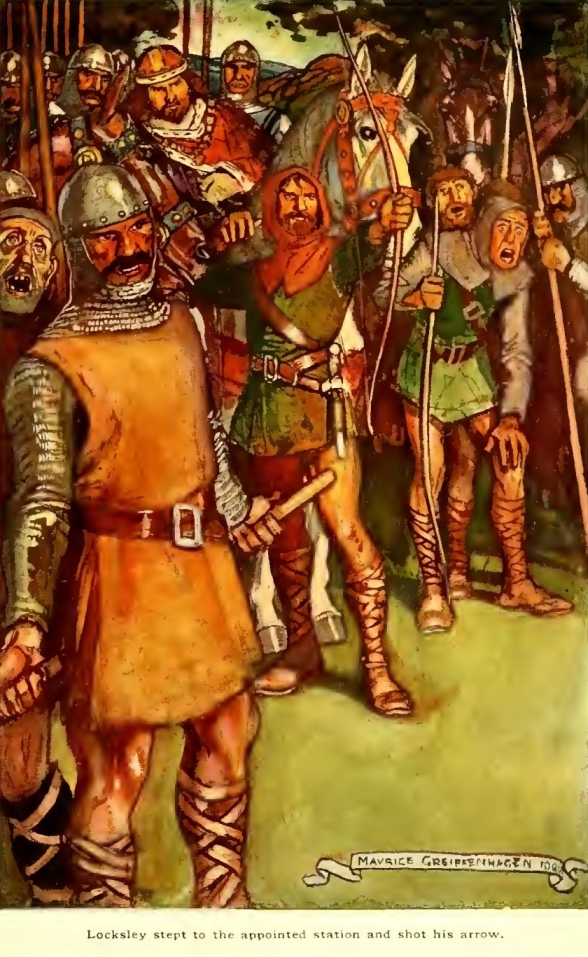
\includegraphics[height=.9\textheight]{ivanhoe/0197m}
    \caption{Locksley stept to the appointed station and shot his arrow.}
\end{figure}

``By the light of heaven!'' said Prince John to Hubert, ``an thou suffer
that runagate knave to overcome thee, thou art worthy of the gallows!''

Hubert had but one set speech for all occasions. ``An your highness were
to hang me,'' he said, ``a man can but do his best. Nevertheless, my
grandsire drew a good bow--''

``The foul fiend on thy grandsire and all his generation!'' interrupted
John, ``shoot, knave, and shoot thy best, or it shall be the worse for
thee!''

Thus exhorted, Hubert resumed his place, and not neglecting the caution
which he had received from his adversary, he made the necessary
allowance for a very light air of wind, which had just arisen, and shot
so successfully that his arrow alighted in the very centre of the
target.

``A Hubert! a Hubert!'' shouted the populace, more interested in a known
person than in a stranger. ``In the clout!--in the clout!--a Hubert for
ever!''

``Thou canst not mend that shot, Locksley,'' said the Prince, with an
insulting smile.

``I will notch his shaft for him, however,'' replied Locksley.

And letting fly his arrow with a little more precaution than before, it
lighted right upon that of his competitor, which it split to shivers.
The people who stood around were so astonished at his wonderful
dexterity, that they could not even give vent to their surprise in their
usual clamour. ``This must be the devil, and no man of flesh and
blood,'' whispered the yeomen to each other; ``such archery was never
seen since a bow was first bent in Britain.''

``And now,'' said Locksley, ``I will crave your Grace's permission to
plant such a mark as is used in the North Country; and welcome every
brave yeoman who shall try a shot at it to win a smile from the bonny
lass he loves best.''

He then turned to leave the lists. ``Let your guards attend me,'' he
said, ``if you please--I go but to cut a rod from the next
willow-bush.''

Prince John made a signal that some attendants should follow him in case
of his escape: but the cry of ``Shame! shame!'' which burst from the
multitude, induced him to alter his ungenerous purpose.

Locksley returned almost instantly with a willow wand about six feet in
length, perfectly straight, and rather thicker than a man's thumb. He
began to peel this with great composure, observing at the same time,
that to ask a good woodsman to shoot at a target so broad as had
hitherto been used, was to put shame upon his skill. ``For his own
part,'' he said, ``and in the land where he was bred, men would as soon
take for their mark King Arthur's round-table, which held sixty knights
around it. A child of seven years old,'' he said, ``might hit yonder
target with a headless shaft; but,'' added he, walking deliberately to
the other end of the lists, and sticking the willow wand upright in the
ground, ``he that hits that rod at five-score yards, I call him an
archer fit to bear both bow and quiver before a king, an it were the
stout King Richard himself.''

``My grandsire,'' said Hubert, ``drew a good bow at the battle of
Hastings, and never shot at such a mark in his life--and neither will I.
If this yeoman can cleave that rod, I give him the bucklers--or rather,
I yield to the devil that is in his jerkin, and not to any human skill;
a man can but do his best, and I will not shoot where I am sure to miss.
I might as well shoot at the edge of our parson's whittle, or at a wheat
straw, or at a sunbeam, as at a twinkling white streak which I can
hardly see.''

``Cowardly dog!'' said Prince John.--``Sirrah Locksley, do thou shoot;
but, if thou hittest such a mark, I will say thou art the first man ever
did so. However it be, thou shalt not crow over us with a mere show of
superior skill.''

``I will do my best, as Hubert says,'' answered Locksley; ``no man can
do more.''

So saying, he again bent his bow, but on the present occasion looked
with attention to his weapon, and changed the string, which he thought
was no longer truly round, having been a little frayed by the two former
shots. He then took his aim with some deliberation, and the multitude
awaited the event in breathless silence. The archer vindicated their
opinion of his skill: his arrow split the willow rod against which it
was aimed. A jubilee of acclamations followed; and even Prince John, in
admiration of Locksley's skill, lost for an instant his dislike to his
person. ``These twenty nobles,'' he said, ``which, with the bugle, thou
hast fairly won, are thine own; we will make them fifty, if thou wilt
take livery and service with us as a yeoman of our body guard, and be
near to our person. For never did so strong a hand bend a bow, or so
true an eye direct a shaft.''

``Pardon me, noble Prince,'' said Locksley; ``but I have vowed, that if
ever I take service, it should be with your royal brother King Richard.
These twenty nobles I leave to Hubert, who has this day drawn as brave a
bow as his grandsire did at Hastings. Had his modesty not refused the
trial, he would have hit the wand as well I.''

Hubert shook his head as he received with reluctance the bounty of the
stranger, and Locksley, anxious to escape further observation, mixed
with the crowd, and was seen no more.

The victorious archer would not perhaps have escaped John's attention so
easily, had not that Prince had other subjects of anxious and more
important meditation pressing upon his mind at that instant. He called
upon his chamberlain as he gave the signal for retiring from the lists,
and commanded him instantly to gallop to Ashby, and seek out Isaac the
Jew. ``Tell the dog,'' he said, ``to send me, before sun-down, two
thousand crowns. He knows the security; but thou mayst show him this
ring for a token. The rest of the money must be paid at York within six
days. If he neglects, I will have the unbelieving villain's head. Look
that thou pass him not on the way; for the circumcised slave was
displaying his stolen finery amongst us.''

So saying, the Prince resumed his horse, and returned to Ashby, the
whole crowd breaking up and dispersing upon his retreat.
